\documentclass{article}
\usepackage[utf8]{inputenc}
\usepackage[a4paper, total={6.5in, 9.5in}]{geometry}
\usepackage{hyperref}
\usepackage{amsmath, amssymb, dsfont}
\usepackage{mathtools}
\usepackage{chemfig}
\usepackage{chemformula}
\usepackage{xcolor}
\definecolor{gray07}{gray}{0.7}
\usepackage{float}
\usepackage{enumitem}
\usepackage{cancel}
\usepackage{pgfplots}
\usepgfplotslibrary{units} % to add units easily to axis
\usepgfplotslibrary{fillbetween} % to fill inbetween curves
\usepgfplotslibrary{colormaps} % to create colormaps
\pgfplotsset{width=12.2cm, height=7cm}
\pgfplotsset{compat=newest} %(making it only compatalbe with
%new releases of pgfplots)
\pgfdeclarehorizontalshading{visiblelight}{50bp}{
color(0.00000000000000bp)=(violet);
color(8.33333333333333bp)=(blue);
color(16.66666666666670bp)=(cyan);
color(25.00000000000000bp)=(green);
color(33.33333333333330bp)=(yellow);
color(41.66666666666670bp)=(orange);
color(50.00000000000000bp)=(red)
}%
\usepackage{tikz}
\usetikzlibrary{decorations.pathreplacing}
\usepackage{multirow}
\usepackage{caption}
\usepackage[load-configurations = abbreviations]{siunitx}
\sisetup{inter-unit-product=\ensuremath{{}\cdot{}}, exponent-product=\ensuremath{{}\cdot{}}, group-minimum-digits=3, range-phrase=-, range-units=single}
\usepackage{graphicx}
\graphicspath{ {./} }
\usetikzlibrary{shapes.arrows}
\let\ce\ch
\newcommand{\bit}{\text{bit}}
\newcommand{\equilibrium}[2]{$\ce{#1}\rightleftharpoons\ce{#2}$}
\newcommand{\soom}{\stackrel{10}{=}}
\newcommand{\vect}{\overrightarrow}
\newcommand{\formulaPyramidFactory}[4]{
    \begin{tikzpicture}[scale=1.25]
\draw (0,0) -- (-0.5, -0.75) node  [align=center, fill=white, midway] {\footnotesize \---};
\draw (0,0) -- (0.5, -0.75) node [align=center, fill=white, midway] {\footnotesize \---};
\draw (0.5, -0.75) -- (-0.5, -0.75) node [align=center, fill=white, midway] {\footnotesize #4};

\draw (0,0) node [above, fill=white] {#1};
\draw (-0.5, -0.75) node [left, fill=white] {#2};
\draw (0.5, -0.75) node [right, fill=white] {#3};

%\draw (0, -1) node [below, align=center] {\small (Pyramide de formule)};
\end{tikzpicture}
}
\newcommand{\formulaPyramid}[3]{\formulaPyramidFactory{#1}{#2}{#3}{$\times$}}
\newcommand{\formulaPyramidAdditive}[3]{\formulaPyramidFactory{#1}{#2}{#3}{$+$}}
\newenvironment{definitions}{\begin{description}[leftmargin=!,labelwidth=\widthof{\bfseries Lorem ipsum dolor}]}{\end{description}}
\newcommand{\deftable}[2]{%
%\hline
\begin{table}[h]
    \centering
    \begin{tabular}{llp{100mm}}%
        %& unité/type & Explication \\ \hline
        #1
    \end{tabular}
    \label{tab:#2_units}
\end{table}%
}
\newcommand{\deftablevar}[3]{%
    $#1$ & $\si{#2}$ & #3 \\
}
\newcommand{\deftableobj}[3]{%
    $#1$ & \textit{#2} & #3 \\
}

\begin{document}

\begin{titlepage}
\begin{center}
\textit{\today}
\vfill
\textbf{\LARGE{Condensé de la terminale}\\\Large{Physique}}\\
\vfill
\large{Ewen Le Bihan\\TS3}
\end{center}
\end{titlepage}
\section*{Notations non vues en cours}
\begin{tabular}{c|l}
	$:=$ & Égal par définition\\
	$\lceil x \rceil$ & Arrondir $x$ à l'entier supérieur. ($\lceil 5.1 \rceil = 6$)\\
	$1.5$ & Séparateur ,\\
	$x\cdot y$ & Multiplication $\times$\\
	$a \propto b$ & $a$ proportionnel à $b$\\
	$a \soom b$ & $a$ même ordre de grandeur que $b$
\end{tabular}
\subsection*{Notations inventées}
\subsubsection*{Pyramides de formules}
\begin{center}
    \formulaPyramid{A}{B}{C} 
\\$\iff A = B\cdot C\quad B = A/C\quad C = A/B$\\
\vspace{30pt}
    \formulaPyramidAdditive{A}{B}{C} 
\\$\iff A = B + C\quad B = A-C\quad C = A - B$\\
\end{center}
\pagestyle{empty}
\newpage
\tableofcontents
\pagestyle{empty}
\newpage

\setcounter{section}{-1}
\section{Outils}
\subsection{La fonction $\log$}

\begin{equation*}
    \begin{split}
        \log (10^x) &= x \quad \text{(réciproque de $\log$)}\\
        \log (a \cdot b) &= \log (a) + \log (b) \\
        \log (\frac{a}{b}) &= \log (a) - \log (b) \\
        \log (a^b) &= b \cdot \log (a)\\
    \end{split}
\end{equation*}
\subsection{L'incertitude $a \pm b$}
On prend la même unité de précision pour $b$ que pour $a$:

$$\cancel{89,79 \pm \SI{4,5}{\micro\meter}} \quad\to\quad 90 \pm \SI{5}{\micro\meter}$$


\newpage
\section{Ondes}

\subsection{Divers infos}

\begin{itemize}
    \item Sur Terre, l'atmosphère \textit{absorbe} certains rayons et il faut utiliser des satellites pour pouvoir les capter (qui sont en dehors de l'atmosphère)
\end{itemize}

\subsection{Définitions}

\begin{definitions}
\item[Onde]
Phénomène de propagation d'une perturbation sans transport de matière
\item[Onde mécanique]
Onde qui se propage dans un milieu physique
\item[Onde électromagnétique]
Onde du spectre électromagnétique pouvant se propager dans le vide
\item[Spectre d'émission]
Spectre représentant des ondes électromagnétiques émises
\item[Spectre continu]
Spectre composé de plages de fréquences
\item[Spectre à raies]
Spectre composé de une ou plusieurs fréquences discrètes
\item[Onde transversale]
Propagation $\to$ \& $\bot$ déformation
\item[Onde longitudinale]
Propagation $\to$
\item[Front d'onde] 
Point "devant" la déformation
\item[Onde progressive]
Onde qui avance
\end{definitions}


\subsection{Les ondes sonores}
\begin{definitions}
\item[Nature] mécanique
\item[Propagation] horizontale
\end{definitions}
\subsubsection{Unité de mesure: Le décibel dB}
$$L = 10 \log \left (\frac{I}{I_0} \right )$$
$$I = I_0 \cdot 10^{L / 10}$$
$$2I = L + 3$$

\begin{definitions}
\item[$I_0$] [$\SI{1E-12}{\watt\per\meter\squared}$] Seuil d'audibilité moyen des humains à $\SI{1}{\kilo\hertz}$
\item[$L$]   [dB] Niveau d'intensité sonore
\item[$I$]   [\si{\watt\per\meter\squared}] Intensité sonore
\end{definitions}

\subsection{Domaines d'ondes électromagnétique}

\begin{table}[h]
    \centering
    \begin{tabular}{r||c|c|c|c|c|c|c}
         Domaine & $\gamma$ & X & UV & Visible & IR & $\mu$-ondes & Radio \\\hline
         $\lambda < $ & $10^{-11}$ &  $10^{-8}$ & $600\cdot10^{-6}$  & $800\cdot10^{-6}$ & $10^{-3}$ & $10^{-1}$ & $+\infty$ \\
         Ex. émetteur & & Radios médicales & Soleil & & Télécommandes & & 
    \end{tabular}
\end{table}

\subsection{Propagation des ondes mécaniques}

\begin{description}
\item[Trajectoire] toutes les directions qui sont offertes
\item[Vitesse de propagation] $\propto$ densité du milieu
\end{description}

\subsection{Le retard $\tau$}
\begin{center}
    \formulaPyramid{$SM$}{$\tau$}{$v$}
\end{center}
\deftable{
    \deftablevar{SM}{\meter}{Distance source (S)-point étudié (M)}
    \deftablevar{v}{\meter\per\second}{Célérité}
    \deftablevar{\tau}{\second}{Retard de l'onde}
}{ondes_retard}

\subsection{Le son}

\begin{definitions}
\item[Type d'onde] Mécanique
\item[Hauteur] Dépend de la fréquence fondamentale. Caractère grave ($f$ faible) / aigu ($f$ élevé)
\item[Timbre] Dépend de la forme du signal (amplitude, nombre et positions des fréquences harmoniques)
\item[Analyse de Fourier] Représentation de l'amplitude de chaque fréquence du signal
\item[Domaine audible] $\SIrange{20}{20 000}{\hertz}$
\end{definitions}

\subsection{L'effet Doppler}

$$f_r = f_e \frac{v_r}{v_r \pm v_e}$$

\deftable{
    \deftablevar{f_r}{\hertz}{Fréquence à la réception}
    \deftablevar{f_e}{\hertz}{Fréquence à l'émission}
    \deftablevar{v_e}{\meter\per\second}{Vitesse de l'émetteur par rapport au récepteur}
    \deftablevar{v_r}{\meter\per\second}{Vitesse de l'onde dans le milieu}
    \deftableobj{\pm}{opérateur}{
        $+$ quand l'émetteur s'éloigne, $-$ quand il se rapproche
    }
}{doppler}

\subsection{Dualité onde-particule}

Chaque objet dans l'univers est à la fois corpusculaire (particule) et une longueur d'onde.

$$\lambda = \frac{h}{p} = \frac{h}{mv}$$

\deftable{
    \deftablevar{\lambda}{\meter}{Longueur d'onde}
    \deftablevar{h}{\SI{6.63E-34}{\joule\per\second}}{Constance de Planck}
    \deftablevar{p}{\kilo\gram\meter\per\second}{Quantité de mouvement}
    \deftablevar{m}{\kilo\gram}{Masse}
    \deftablevar{v}{\meter\per\second}{Vitesse}
}{broglie}

\newpage

\section{Transferts d'énergie thermique \& mécanique}
Fil 1 〉 Séq 3 〉 Part. A

\subsection{Définitions}
\begin{definitions}
\item[Convection]
Transfert thermique entre fluides

\item[Conduction]
Transfert thermique par contact physique

\item[Rayonnement]
Transfert thermique par émission d'ondes électromagnétiques

\item[Conducteur]
Matériau favorisant les transferts par conduction

\item[Isolant]
Matériau limitant les transferts par conduction
\end{definitions}

\subsection{Flux thermique $\Phi$}

\begin{center}
    \formulaPyramid{Q}{$\Phi$}{$t$}
\end{center}

\deftable{
    \deftablevar{\Phi}{\watt}{Flux}
    \deftablevar{Q}{\joule}{Transfert thermique}
    \deftablevar{t}{\second}{Durée du transfert}
}{flux_thermique}

\subsection{Résistance thermique $R_\text{th}$}

\begin{center}
    \formulaPyramid{$\Delta T$}{$R_\text{th}$}{$\Phi$}
    \formulaPyramid{$e$}{$R_\text{th}$}{$\lambda s$}
\end{center}

\deftable{
    \deftablevar{R_{\text{th}}}{\kelvin\per\watt}{Résistance thermique}
    \deftableobj{\Delta T}{\si{\kelvin} ou \si{\celsius}}{Écart de temp. entre les deux matériaux}
    \deftablevar{\Phi}{\watt}{Flux thermique}
    \deftablevar{e}{\meter}{Épaisseur}
    \deftablevar{s}{\meter\squared}{Surface}
    \deftablevar{\lambda}{\watt\per\meter\per\kelvin}{Conductivité thermique}
}{resistance_thermique}

\subsection{Énergie interne $U$}

Somme des énergies microscopiques de toutes les particules

$$\Delta U = m \cdot c \cdot \Delta T$$

\deftable{
    \deftablevar{\Delta U}{\joule}{Variation d'énergie interne}
    \deftablevar{m}{\kilo\gram}{Masse}
    \deftablevar{c}{\joule\per\kilo\gram\per\kelvin}{Capacité thermique massique du solide}
    \deftableobj{\Delta T}{\si{\kelvin} ou \si{\celsius}}{Écart de temp. entre les deux matériaux}
}{energie_interne}

\subsection{Bilan énergétique}
\subsubsection{Méthode}

\begin{enumerate}
    \item \textit{Définir le système macroscopique étudié}\\
        Des fois mis entre \{\} dans l'énoncé
    \item \textit{Repérer les modes de transfert}\\
        \begin{definitions}
            \item[Thermique] chaleur Q
            \item[Mécanique] travail W
        \end{definitions}
    \item \textit{Affecter un signe aux transferts}\\
        \begin{definitions}
            \item[E reçue] $+$
            \item[E cédée] $-$
        \end{definitions}
\end{enumerate}

\subsubsection{Example}

\begin{center}
    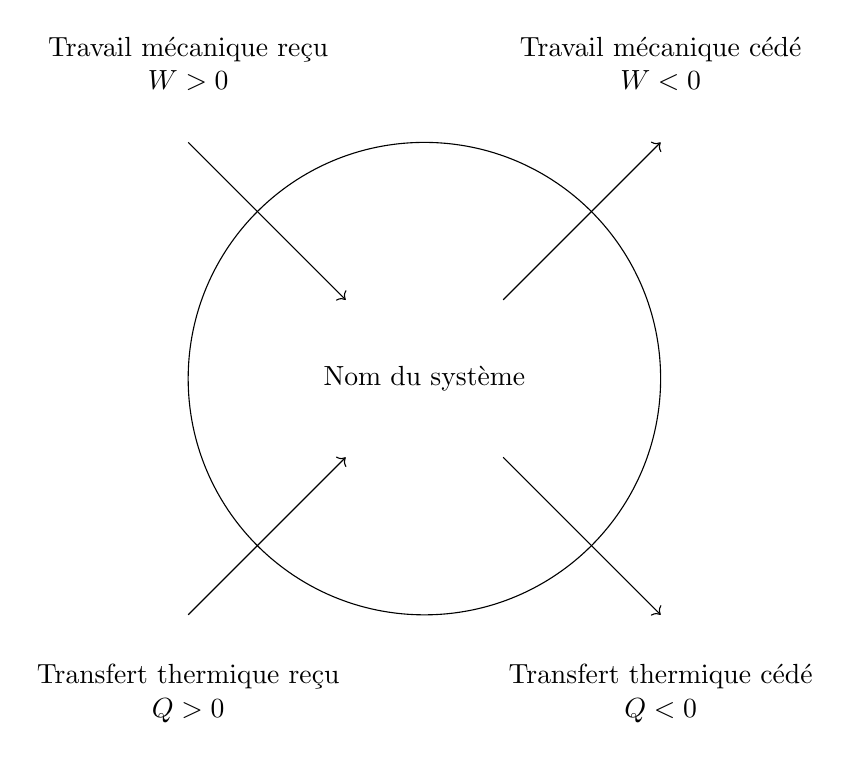
\begin{tikzpicture}
\draw (0,0) circle (3);
\draw (0,0) node [midway] {Nom du système};

\draw[->] (-3,-3) -- (-1,-1);
\draw (-3, -4) node [align=center, fill=white] {Transfert thermique reçu \\ $Q > 0$};

\draw[->] (-3, 3) -- (-1,1);
\draw (-3, 4) node [align=center, fill=white] {Travail mécanique reçu \\ $W > 0$};

\draw[<-] (3, -3) -- (1,-1);
\draw (3, -4) node [align=center, fill=white] {Transfert thermique cédé \\ $Q < 0$};

\draw[<-] (3,3) -- (1,1);
\draw (3, 4) node [align=center, fill=white] {Travail mécanique cédé \\ $W < 0$};
\end{tikzpicture}
\end{center}

\subsection{Différentes énergies}

\begin{center}
    \begin{tikzpicture}[scale=0.75]
\draw (0,0) -- (-6, -6);
\draw (0,0) -- (6, -6);

\draw (-6,-6) -- (-9, -12);
\draw (-6,-6) -- (-3, -12);
\draw (6,-6) -- (9, -12);
\draw (6,-6) -- (3, -12);

\draw (0,0) node [align=center, fill=white] {$E_T$ \\ Énergie totale \\ $\Delta E_T = W + Q$};

\draw (-6, -6) node [align=center, fill=white] {$E_m$ \\ Macroscopique};
\draw (6, -6) node [align=center, fill=white] {$U$ \\ Microscopique \\ atomes, molécules, ions};

\draw (-9, -12) node [align=center, fill=white] {$E_{\text{c, macro}}$ \\ Cinétique \\ $ = \frac{1}{2} m v^2$};
\draw (-3, -12) node [align=center, fill=white] {$E_{pp}$ \\ Potentielle \\ $ = m g z$};
\draw (3, -12) node [align=center, fill=white] {$\Sigma E_{\text{c, micro}}$ \\ Cinétique \\ $ \propto \text{vitesse des particules}$};
\draw (9, -12) node [align=center, fill=white] {$\Sigma U_p$ \\ Potentielle \\ $ \propto \text{distance inter-particule}$};
\end{tikzpicture}
\end{center}

\subsection{Lois des circuits en série \& en dérivation}



\newpage 

\section{Transferts d'énergie quantique}
Fil 1 〉 Séq 3 〉 Part. B

\subsection{Définitions}
\begin{definitions}
 \item[Quantifié] ne peut prendre que des valeurs discrètes déterminées
 \item[État fondamental] Niveau d'énergie le plus bas ($E_0$)
 \item[Atome excité] dans un niveau d'énergie autre que l'état fondamental
 \item[Atome stable] dans l'état fondamental
 \item[Transition quantique] Passage d'un état à un autre
\end{definitions}

\subsection{Propriétés d'un laser}
\begin{definitions}
\item[Monochromatique] Une seule couleur
\item[Faisceau lumineux directif] Faisceau dans une seule direction
\end{definitions}

\subsection{Au niveau atomique}
\subsubsection{Diagramme d'énergie}
 \begin{center}
     Example: l'atome de Sodium \\ 
\begin{tikzpicture}[scale=1.5]
\draw[->,>=latex] (0, -5.2) -- (0, 2);
\draw (-0.5, 1.75) node {$E$ (\si{eV})};

\draw (0, -5.14) -- (5, -5.14);
\draw (-0.2, -5.14) node [left] {$-5.14$};
\draw (5.2, -5.14) node [right] {$n = 0$  (état fondamental)};

\draw (0, -3.03) -- (5, -3.03);
\draw (-0.2, -3.03) node [left] {$-3.03$};
\draw (5.2, -3.03) node [right] {$n = 1$};

\draw (0, -1.93) -- (5, -1.93);
\draw (-0.2, -1.93) node [left] {$-1.93$};
\draw (5.2, -1.93) node [right] {$n = 2$};

\draw (0, -1.51) -- (5, -1.51);
\draw (-0.2, -1.51) node [left] {$-1.51$};
\draw (5.2, -1.51) node [right] {$n = 3$};

\draw (0, -1.38) -- (5, -1.38);
\draw (-0.2, -1.18) -- (0, -1.38);
\draw (-0.2, -1.18) node [left] {$-1.38$};
\draw (5.2, -1.18) -- (5, -1.38);
\draw (5.2, -1.18) node [right] {$n = 4$};

\draw (0, 0.80) -- (5, 0.80);
\draw (-0.2, 0.80) node [left] {$0.80$};
\draw (5.2, 0.80) node [right] {$n = 5$};

\draw[->] (2.5, 0.80) -- (2.5, -3.03);
\draw (3.75, -1) node [above] {photon};
\draw[->, line join=round,
decorate, decoration={
    zigzag,
    segment length=4,
    amplitude=.9,post=lineto,
    post length=2pt
}] (3, -1) -- (4.5, -1);
\end{tikzpicture}

 \end{center}
\subsubsection{Calcul de l'énergie d'un transfert}
\begin{samepage}
\begin{center}
    \formulaPyramid{$E$}{$h$}{$\nu = \dfrac{c}{\lambda}$}
\end{center}
\begin{definitions}
\item[h] [$\approx \:  \SI{6E-34}{\joule\per\second}$] Constante de planck
\item[c] [$\approx  \: \SI{3E8}{\meter\per\second}$] Célérité de la lumière dans le vide
\item[\lambda] [\si{\meter}] Longueur d'onde
\end{definitions}
\end{samepage}

\subsubsection{Absorption}

\begin{definitions}
\item[Devient] excité
\item[Photon] $1 \: \text{(avant)} \longrightarrow 0  \:  \text{(après)}$
\item[Moment] quand le photon touche l'atome
\end{definitions}

\subsubsection{Émission spontanée}

\begin{definitions}
\item[Devient] stable
\item[Photon] $0 \longrightarrow 1$
\item[Moment] aléatoire
\item[Trajectoire] aléatoire
\end{definitions}

\subsubsection{Émission stimulée}

\begin{definitions}
\item[Devient] stable
\item[Photon] $1 \longrightarrow 2$
\item[Moment] $\quad$ % Trick to keep the list below the \item
    \begin{itemize}
        \item L'atome est déjà stimulé avant la collision
        \item Un photon touche l'atome
    \end{itemize}
\item[Trajectoire] celle du photon incident
\end{definitions}

\subsection{Au niveau moléculaire}

Au niveau moléculaire il y a des \textbf{sous-niveaux vibratoires}, car les atomes vibrent les uns par rapport aux autres.

\subsection{Domaines spectraux des transitions}
\begin{table}[h]
    \centering
    \begin{tabular}{c|c|c}
         Nature de l'énergie & Énergie absorbée [$\si{\eV}$] & Domaine spectral associé \\
         \hline
         Électronique & $\in [1.5 ; 10]$ & Visible, ultraviolet \\
         Vibratoire & $\in [0.003  ; 1.5]$ & Infrarouge
    \end{tabular}
    \label{tab:spectral_domains}
\end{table}

\newpage

\section{Réaction acido-basiques}

\subsection{Définitions}

\begin{definitions}

\item[Acide]
Espèce chimique capable de \textbf{céder} au moins un proton $\ce{H^+}$ au cours d’une réaction.

\item[Base]
Espèce chimique capable de \textbf{capter} au moins un proton $\ce{H^+}$ au cours d’une réaction.

\item[Acide ou base fort(e)]
Acide/base qui réagit totalement avec l'eau

\item[Solution tampon]
Solution qui compense les changements de pH, son pH ne peut varier que très peu.

\item[Exothermique]
Qui dégage de la chaleur

\item[Endothermique]
Qui absorbe de la chaleur (Endotre thermes (haha), qui "dégage du froid")

\end{definitions}

\subsection{Le potentiel hydrogène $\text{pH}$}

\subsubsection{Contrôle du pH}
Important pour le sang

\subsubsection{Papier pH}
Déposer une goutte du produit sur la papier pH (ne pas tremper le papier dans la solution)
\begin{definitions}
\item[Précision] $\pm 1$
\end{definitions}

\subsubsection{pH-mètre}
Étalonner avec des solutions tampons
\begin{definitions}
\item[Précision] $\pm 0,1$
\end{definitions}

\subsubsection{Indicateur coloré}
Solutions avec zones de pH associées à couleurs. Ne marche que si la solution à mesurer est incolore ou blanche
\begin{enumerate}
    \item Verser indicateur dans solution
    \item Couleur de solution inconnue $\implies$ encadrement de la valeur
\end{enumerate}
\begin{definitions}
\item[Précision] Dépend de la solution. Pas de valeurs exactes.
\end{definitions}

\subsubsection{Calcul}

Quand on fait un calcul avec cette grandeur, la précision maximale est de \textbf{un seul chiffre après la virgule}
\vspace{5pt}

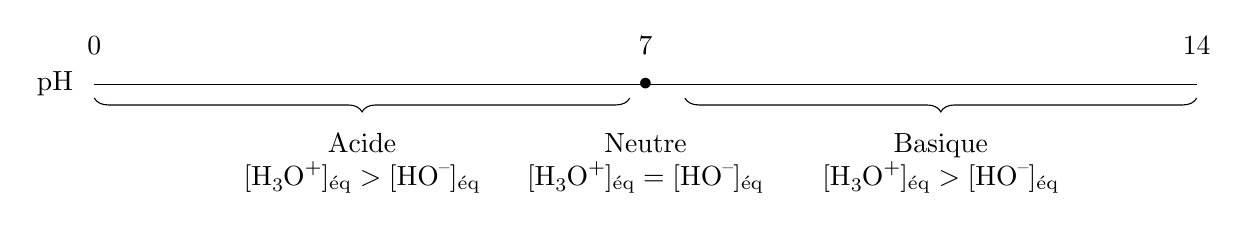
\begin{tikzpicture}
\draw (-7.5, 0) node {pH};
\draw (-7, 0) -- (7, 0);
\draw (-7, 0) node [above=0.25cm] {0};
\draw (0, 0) node [above=0.25cm] {7};
\draw (7, 0) node [above=0.25cm] {14};

\draw[decorate, decoration={brace, mirror, amplitude=5pt, raise=5pt}] (-7, 0) -- (-0.2, 0) node [midway, below=0.5cm, align=center] {Acide\\$[\ce{H3O^+}]_\text{éq} > [\ce{HO^-}]_\text{éq}$};
\draw (0, 0) node {$\bullet$};
\draw (0, 0) node [below=0.5cm,  align=center] {Neutre\\$[\ce{H3O^+}]_\text{éq} = [\ce{HO^-}]_\text{éq}$};
\draw[decorate, decoration={brace, mirror, amplitude=5pt, raise=5pt}] (0.5, 0) -- (7, 0) node [midway, below=0.5cm,  align=center] {Basique\\$[\ce{H3O^+}]_\text{éq} > [\ce{HO^-}]_\text{éq}$};
\end{tikzpicture}


\begin{equation*}
    \begin{split}
        \text{pH} &= -\log [\ce{H3O^+}] \\
                  &= -\log C\quad\quad\quad\quad\quad\:\:\text{(pour les acides forts)} \\
                  &= 14 + \log C\quad\quad\quad\quad\:\text{(pour les bases fortes)} \\
                  &= \text{p}K_a + \log \frac{[\ce{A^-}]_\text{éq}}{[\ce{HA}]_\text{éq}}\quad\text{(preuve: voir 4.6)}
    \end{split}
\end{equation*}

\ce{[X]} désigne la concentration molaire de l'ion \ce{X} en \si{\mol\per\liter}

\subsection{Réactions acido-basique}

Sauf en présence d'acide/base fort(e)s, la réaction n'est pas totale, c'est un équilibre.\\
Soit $\ce{HA}$ un acide quelconque.\\
$$\ce{HA} \rightleftharpoons \underbrace{\ce{A^-}}_{\mathclap{\text{Base conjuguée}}} +\; \ce{H^+}$$
Mélange avec de l'eau:
\begin{center}
    \equilibrium{HA_{(aq)} + H2O_{(l)}}{A^{-}_{(aq)} + H3O^{+}_{(aq)}}
\end{center}
\\
Avec un acide fort, la réaction est complète:
$$\ce{HA -> A^- + H^+}$$

\subsection{Réactions base forte ou acide fort}
\begin{itemize}
    \item Besoin de hotte aspirante
    \item Exothermique
\end{itemize}

\subsection{Produit ionique de l'eau $K_e$}
Pour toutes les solutions:

$$K_e = [\ce{H3O^+}]_\text{éq} \cdot [\ce{HO^-}]_\text{éq} = 10^{14}\quad\text{(à 25°C)}$$

\subsection{Constantes d'acidité $\text{p}K_a$ et $K_a$}

$$K_a = \frac{[\ce{A^-}]_\text{éq} \cdot [\ce{H3O^+}]_\text{éq}}{[\ce{AH}]_\text{éq}}$$
$$\text{p}K_a = -\log K_a$$

$$\text{p}K_a \in [0 ; 14]\quad\text{pour les couples acide faible/base faible}$$

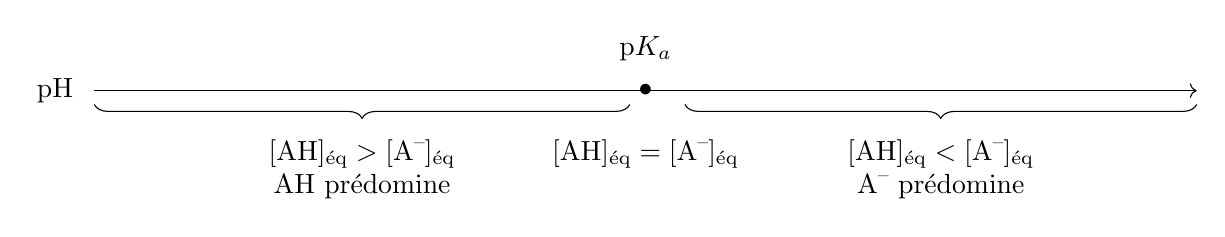
\begin{tikzpicture}
\draw (-7.5, 0) node {pH};
\draw [->] (-7, 0) -- (7, 0);
\draw (0, 0) node [above=0.25cm] {p$K_a$};

\draw[decorate, decoration={brace, mirror, amplitude=5pt, raise=5pt}] (-7, 0) -- (-0.2, 0) node [midway, below=0.5cm, align=center] {$[\ce{AH}]_\text{éq} > [\ce{A^-}]_\text{éq}$\\\ce{AH} prédomine};
\draw (0, 0) node {$\bullet$};
\draw (0, 0) node [below=0.5cm, align=center] {$[\ce{AH}]_\text{éq} = [\ce{A^-}]_\text{éq}$};
\draw[decorate, decoration={brace, mirror, amplitude=5pt, raise=5pt}] (0.5, 0) -- (7, 0) node [midway, below=0.5cm, align=center] {$[\ce{AH}]_\text{éq} < [\ce{A^-}]_\text{éq}$\\\ce{A^-} prédomine};
\end{tikzpicture}

\subsection{Preuve de $\text{pH} = pK_a + \log \frac{[\ce{A^-}]_\text{éq}}{[\ce{HA}]_\text{éq}}$}
\label{sec:proofPhEqPkaPlusLog}

\begin{equation*}
    \begin{split}
        -\log pK_a &= -\log \left (  \frac{[\ce{A^-}]_\text{éq}\cdot[\ce{H3O^+}]_\text{éq}}{[\ce{HA}]_\text{éq}} \right ) \\
        & \textcolor{gray07}{ \log\left( \frac{a}{b} \right) = \log(b) - \log(a) } \\
        pK_a &= -\log \frac{[\ce{A^-}]_\text{éq}}{[\ce{HA}]_\text{éq}} -\log [\ce{H3O^+}]_\text{éq} \\
            &= -\log \frac{[\ce{A^-}]_\text{éq}}{[\ce{HA}]_\text{éq}} + \text{pH} \\
        \text{pH} &= pK_a + \log \frac{[\ce{A^-}]_\text{éq}}{[\ce{HA}]_\text{éq}}
    \end{split}
\end{equation*}

%\newpage

%\section{Vérification de concentrations}

\subsection{Loi de Kohlrausch: la conductivité $\sigma$}

\subsubsection{Pour un ion}

\begin{center}
    \formulaPyramid{$\sigma$}{$c$}{$\lambda$}
\end{center}
\deftable{
    \deftablevar{\sigma}{\siemens\per\meter}{Conductivité}
    \deftableobj{c}{$\text{mol}\cdot\text{m}\textcolor{red}{^{-3}}$}{Concentration molaire}
    \deftablevar{\lambda}{\siemens\per\square\meter\per\mol}{Conductivité électrique molaire}
}{conductivite}
\subsubsection{Pour une molécule}
Calcul pour une molécule composés des ions $X$

$$\sigma_{X_1 X_2 X_3 \dots X_j} = \sum_{i=1}^{j} [X_i]\lambda_{X_i}$$

\subsubsection{Example: conductivité de \ce{HO^-Na^+}}

\begin{equation*}
    \begin{split}
        \sigma_{\ce{HO^-Na^+}} &= [\ce{HO-}]\lambda_{\ce{HO-}} + [\ce{Na^+}]\lambda_{\ce{Na^+}} \\
                              &= 2\cdot19.8\cdot10^{-3} + 2\cdot5.0\cdot10^{-3} \\
                              &= \SI{5.0E-2}{\siemens\per\meter} \\
    \end{split}
\end{equation*}


\newpage\section{Optique}

\subsection{Diffraction}

\texttt{TODO: Schéma w/ TikZ}

\begin{center}
    Si $\lambda \soom a$\\
    \formulaPyramid{$\lambda$}{$\theta$}{$a$}
\end{center}

\deftable{
    \deftablevar{\lambda}{\meter}{Longueur d'onde}
    \deftablevar{\theta}{\radian}{Demi-angle de diffraction}
    \deftablevar{a}{\meter}{Largeur de la fente}
}{diffraction}

\subsection{Interférences}

\texttt{TODO: Schéma w/ TikZ}

\begin{center}
    \formulaPyramid{$\lambda D$}{$i$}{$l$}
\end{center}

\deftable{
    \deftablevar{\lambda}{\meter}{Longueur d'onde}
    \deftablevar{D}{\meter}{Distance fente-écran}
    \deftablevar{i}{\meter}{Distance interfrange}
    \deftablevar{l}{\meter}{Distance inter-fentes}
}{interfrange}

$$\delta = d_1 - d_2$$

\deftable{
    \deftablevar{\delta}{\meter}{Différence de marche}
    \deftablevar{d_1}{\meter}{Distance parcourue par le rayon 1}
    \deftablevar{d_2}{\meter}{Distance parcourue par le rayon 2}
}{difference_de_marche}

\begin{definitions}
\item[Constructive] $\exists k \in \mathds{Z}\quad \delta = k \lambda$
\item[Destructives] $\exists k \in \mathds{Z}\quad \delta = \left(k + \frac{1}{2}\right) \lambda$
\end{definitions}

\newpage
\section{Signaux}

\subsection{Types de signaux}

\begin{definitions}
\item[Analogique] Précision infinie. Issues de mesures de phénomènes
\item[Numérique] Précision limitée par le nombre de bits utilisés pour coder l'information.
\end{definitions}

\subsection{Numérisation $A \to D$}

\begin{definitions}
\item[Échantillonage] Prélevage de valeurs à intervalles de temps régulières.
\item[Quantification] Approximation de chaque valeur à sa valeur binaire la plus proche.
\end{definitions}

\deftable{
    \deftablevar{f_e}{\hertz}{Fréquence d'échantillonage}
    \deftablevar{T_e}{\second}{Période d'échantillonage}
    \deftablevar{N}{}{Nombre de mesures}
    \deftablevar{T}{\second}{Période du signal}
    \deftablevar{n}{\bit}{Bits de quantification}
    \deftablevar{q}{}{Plus petite valeur échantillonable}
}{echantillonage_quantification}

\subsection{Transmission}
\subsubsection{Débit binaire $D$}

$$D = \frac{1}{T_B} = Nkf_e$$

\deftable{
    \deftablevar{N}{}{Nombre de signaux}
    \deftablevar{k}{}{Nombre de bits utilisés}
    \deftablevar{D}{\bit\per\second}{Débit binaire}
    \deftablevar{T_B}{\second}{Durée d'un bit}
}{debit_binaire}

\subsubsection{Atténuation}

$$P_\text{reçu} = P_\text{émis} \cdot e^{-\alpha d}$$
\begin{equation*}
    \begin{split}
        A_\text{dB} &= -10 \log \frac{P_\text{reçu}}{P_\text{émis}} \\
        &= \alpha_\text{dB} d
        &> 0
    \end{split}
\end{equation*}

\deftable{
    \deftablevar{\alpha}{}{Coefficient d'atténuation}
    \deftablevar{d}{\meter}{Distance}
    \deftablevar{P_\text{reçu}}{\watt}{Puissance reçue}
    \deftablevar{P_\text{émis}}{\watt}{Puissance émise}
    \deftablevar{A_\text{dB}}{\decibel}{Coefficient d'atténuation}
    \deftablevar{\alpha_\text{dB}}{\decibel}{Atténuation}
}{attenuation}

\subsubsection{Types de câbles}

\begin{center}
    \begin{tikzpicture}[scale=0.75]
\draw (0,0) -- (-6, -6);
\draw (0,0) -- (6, -6);

\draw (-6,-6) -- (-6, -12);
\draw (6,-6) -- (9, -12);
\draw (6,-6) -- (3, -12);

\draw (0,0) node [align=center, fill=white] {Moyens de transmission du signal};

\draw (-6, -6) node [align=center, fill=white] {Transmission guidée};
\draw (6, -6) node [align=center, fill=white] {Transmission non-guidée};

\draw (-6, -12) node [align=center, fill=white] {Ondes électromagnétiques};
\draw (3, -12) node [align=center, fill=white] {Câbles};
\draw (9, -12) node [align=center, fill=white] {Fibre optique};
\end{tikzpicture}
\end{center}

\section{Stockage optique et d'images}
\subsection{Stockage d'une image}
Stockage d'une image en couleur:

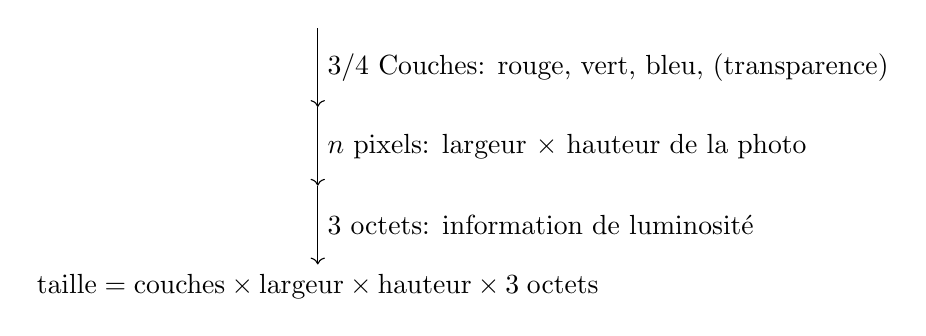
\begin{tikzpicture}
\draw[->] (0,0) -- (0,-1) node[midway, right] { 3/4 Couches: rouge, vert, bleu, (transparence) };
\draw[->] (0,-1) -- (0,-2) node[midway, right] { $n$ pixels: largeur $\times$ hauteur de la photo };
\draw[->] (0,-2) -- (0,-3) node[midway, right] { 3 octets: information de luminosité };
\draw[] (0,-3) node [below] { $\text{taille} = \text{couches}\times\text{largeur}\times\text{hauteur}\times3\;\text{octets}$ };
\end{tikzpicture}

\subsection{Stockage optique}
\subsubsection{Stockage}
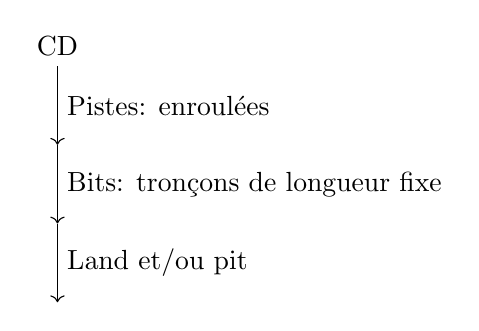
\begin{tikzpicture}
\draw[] (0,0.25) node { CD };
\draw[->] (0,0) -- (0,-1) node[midway, right] { Pistes: enroulées };
\draw[->] (0,-1) -- (0,-2) node[midway, right] { Bits: tronçons de longueur fixe };
\draw[->] (0,-2) -- (0,-3) node[midway, right] { Land et/ou pit };
\end{tikzpicture}

\begin{equation*}
    \begin{split}
        \text{largeur de piste} &\propto \text{nombre de pistes que l'on peut mettre} \\
        &\propto \text{capacité de stockage} \\
        &\propto \lambda \;\text{du laser lecteur} \\
        &\propto \text{NA du laser lecteur}
    \end{split}
\end{equation*}
\subsubsection{Lecture}
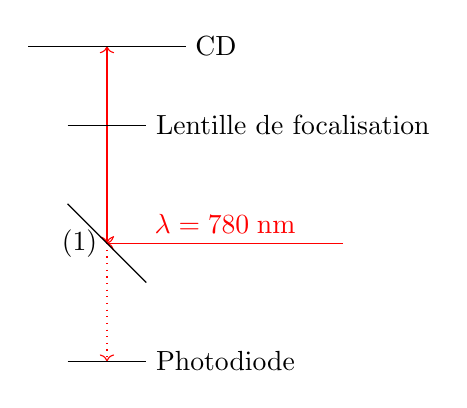
\begin{tikzpicture}
\draw[<->, color=red] (0,0) -- (0,-2.5);
\draw[->, color=red] (3,-2.5) -- (0,-2.5) node [above, midway] { $\lambda = 780\;\text{nm}$ };
\draw[->, dotted, color=red] (0,-2.5) -- (0,-4);

\draw (-1,0) -- (1,0) node [right] { CD };
\draw (-0.5,-1) -- (0.5,-1) node [right] { Lentille de focalisation };
\draw (-0.5,-2) -- (0.5,-3) node [left, midway] { (1) };
\draw (-0.5,-4) -- (0.5,-4) node [right] { Photodiode };
\end{tikzpicture}
\begin{description}
\item[(1)] Mirror semi-transparent
\end{description}

\paragraph{Pour un bit 1}
\begin{enumerate}
    \item Profondeur d'un pit: $\dfrac{\lambda}{4}$
    \item Décalage land/pit: $\dfrac{\lambda}{2}$ (aller\textbf{+}retour)
    \item $\dfrac{\lambda}{2} \implies \text{Interférence destructive}$
    \item Pour la photodiode: Signal $\approx 0$
    \item Transition land/pit $\implies$ 1
\end{enumerate}

\paragraph{Pour un bit 0}
\begin{enumerate}
    \item Signaux initial/après rebond indentiques $\implies \text{Interférence constructive}$
    \item Pour la photodiode: Signal fort
    \item Pas de transition $\implies$ 0
\end{enumerate}

\paragraph{Ouverture numérique $NA$}
.\\

\begin{equation*}
\begin{tabular}{
  @{}
  m{.5\textwidth}
  @{}
  m{.5\textwidth}
  @{}
}
\centering
$\displaystyle
\begin{split}
    NA &= \sin \alpha \\
    &= \frac{0.5D}{\sqrt{(0.5D)^2 + f^2}} \\
    d &= 1.22 \frac{\lambda}{NA}
\end{split}
$
&
\centering
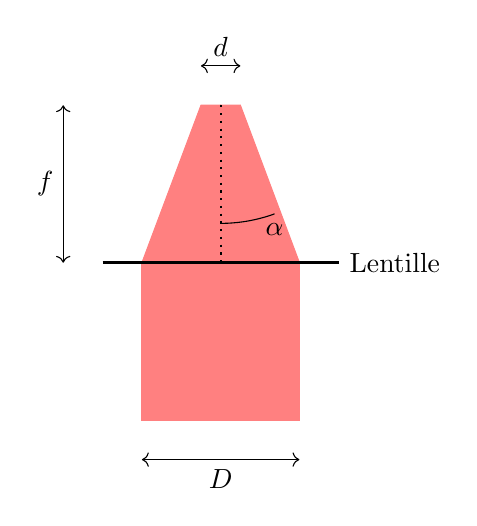
\begin{tikzpicture}

\draw[fill=red!50, color=red!50] (-0.25,0) -- (-1,-2) -- (0,-2) -- (0,0) -- cycle;
\draw[fill=red!50, color=red!50] (0.25,0) -- (1,-2) -- (0,-2) -- (0,0) -- cycle;
\draw[fill=red!50, color=red!50]  (-1,-2) -- (-1,-4) -- (1,-4) -- (1,-2) -- cycle;
\draw[very thick] (-1.5,-2) -- (1.5,-2) node[right] { Lentille };
\draw[thick, dotted] (0,0) -- (0,-2);

\draw (0,-1.5) arc (-90:-70:2) node[below] { $\alpha$ };
\draw[<->] (-0.25,0.5) -- (0.25,0.5) node[midway, above] { $d$ };
\draw[<->] (-1,-4.5) -- (1,-4.5) node[midway, below] { $D$ };
\draw[<->] (-2,-2) -- (-2,0) node[midway, left] { $f$ };

\end{tikzpicture}
\end{tabular}
\end{equation*}

\newpage
\section{Mécanique}
\subsection{Vecteurs du mouvement}
\begin{equation*}
    \begin{split}
        \vec a = \frac{d\vec v}{dt} = \frac{d\frac{d\vect{OM}}{dt}}{dt}
    \end{split}
\end{equation*}

\subsection{Principe d'intertie}

$$
\vec{v} = \vect{\text{cte}} \iff \Sigma \vect{F_{\text{ext}}} = \vec{0} \\
$$

\subsection{Isolation d'un système}
\begin{definitions}
\item[Isolé] $\vec p = m \vec v$
\item[Pseudo-isolé] Les forces se compensent
\end{definitions}

\subsection{Principe fondamental de la dynamique}
\begin{equation*}
    \begin{split}
        \Sigma \vect{F_\text{ext}} &= \frac{d\vec p}{dt} \\
                                   &= m \vec a \quad \text{(si la masse est constante)}
    \end{split}
\end{equation*}

\subsection{Application}

On utilise les conditions initiales:
On nous donne $\alpha$ l'angle de lancement initial.
Pour avoir $v_{_0x}$ et $v_{_0y}$ on calcule les sinus et cosinus de $\alpha$.

Quand la seule force s'appliquant à l'objet en chute est le poids $\vec{P}$, on a:

\begin{equation*}
    \begin{split}
        \Sigma \vect{F_\text{ext}} &= m \vec a \\
        \iff \vec P &= m \vec a\\
        \iff m \vec g &= m \vec a \\
        \iff \vec g &= \vec a
    \end{split}
\end{equation*}

$$
\begin{pmatrix}
a_x \\ a_y
\end{pmatrix} = \begin{pmatrix}
0 \\ -g
\end{pmatrix}
$$

On primitive pour trouver la vitesse puis la position:

$$
\vec v = \begin{cases}
v_x &= C_1 \\
v_y &= -gt + C_2
\end{cases}
$$

On détermine $C_1$ et $C_2$ avec les conditions initiales:

à $t=0$:

$$
\begin{cases}
v_x = C_1 &= v_{_0x} = v_0 \cos \alpha \\
v_y = -gt + C_2 &= 0 + v_{_0y} = v_0 \sin \alpha \\
\end{cases}
$$

Donc: 

$$
\vec v = \begin{cases}
v_x &= v_0 \cos \alpha \\
v_y &= -gt + v_0\sin\alpha
\end{cases}
$$

et:

$$||\vec v|| = \sqrt{v_x^2 + v_y^2}$$

\end{document}